% ─────────────────────────────────────────────────────────────
% ACTIVIDAD 6: Análisis de grupos para detección de anomalías
% ─────────────────────────────────────────────────────────────

La detección de valores anómalos (\emph{outliers} o \emph{anomalies}) es una tarea crítica en analítica de datos, con aplicaciones en detección de fraude, mantenimiento predictivo y seguridad de redes. El análisis de grupos proporciona un marco no supervisado para identificar anomalías sin requerir ejemplos etiquetados de comportamiento anómalo.

% ─────────────────────────────────────────────────────────────
\subsection{Fundamento teórico}
% ─────────────────────────────────────────────────────────────

La premisa fundamental es que los datos normales forman conglomerados densos y coherentes, mientras que las anomalías son puntos que no encajan en ningún cluster o que residen en regiones de muy baja densidad. Formalmente, sea $\mathcal{D} = \{ \mathbf{x}_1, \dots, \mathbf{x}_n \} \subset \mathbb{R}^d$ y sea $\mathcal{C} = \{ C_1, \dots, C_k \}$ una partición obtenida por un algoritmo de clustering. Se definen dos criterios de anomalía~\cite{chandola2009anomaly}:

\begin{enumerate}[label=\arabic*.]
    \item \textbf{Distancia al centroide más cercano:} un punto $\mathbf{x}$ es anómalo si
    \begin{equation}
        \min_{C_j \in \mathcal{C}} \, \mathrm{dist}\bigl(\mathbf{x}, \boldsymbol{\mu}_j\bigr) > \theta,
    \end{equation}
    donde $\boldsymbol{\mu}_j$ es el centroide del cluster $C_j$ y $\theta$ es un umbral predefinido.

    \item \textbf{Densidad local:} en métodos basados en densidad (DBSCAN, HDBSCAN), los puntos clasificados como \emph{ruido} ($\mathrm{label} = -1$) son directamente anómalos.
\end{enumerate}

% ─────────────────────────────────────────────────────────────
\subsection{Enfoque práctico: Clustering + umbral de distancia}
% ─────────────────────────────────────────────────────────────

El procedimiento habitual consta de tres etapas:

\begin{enumerate}[label=\arabic*.]
    \item \textbf{Agrupar} los datos con un algoritmo adecuado (por ejemplo, $k$-means).
    \item \textbf{Calcular} para cada punto su distancia al centroide de su cluster asignado.
    \item \textbf{Marcar} como anómalo todo punto cuya distancia exceda un percentil alto (típicamente el percentil 95 o 99) de la distribución de distancias.
\end{enumerate}

\begin{figure}[H]
    \centering
    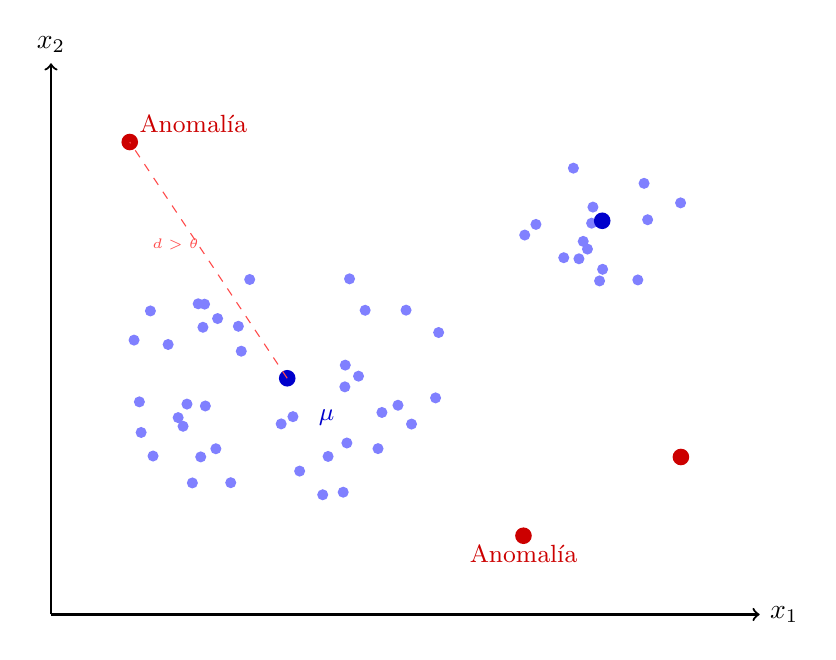
\begin{tikzpicture}[scale=1.0]
        % Cluster principal (normal)
        \foreach \i in {1,...,40} {
            \pgfmathsetmacro{\x}{3.0+rand*2.0}
            \pgfmathsetmacro{\y}{3.0+rand*1.5}
            \fill[blue!50] (\x,\y) circle (2pt);
        }
        % Centroide
        \fill[blue!80!black] (3,3) circle (3pt);
        \node[blue!80!black, font=\small] at (3.5,2.5) {$\boldsymbol{\mu}$};

        % Pequeño cluster secundario (también normal)
        \foreach \i in {1,...,15} {
            \pgfmathsetmacro{\x}{7.0+rand*1.0}
            \pgfmathsetmacro{\y}{5.0+rand*0.8}
            \fill[blue!50] (\x,\y) circle (2pt);
        }
        \fill[blue!80!black] (7,5) circle (3pt);

        % Outliers
        \fill[red!80!black] (1,6) circle (3pt) node[above right, font=\small] {Anomalía};
        \fill[red!80!black] (6,1) circle (3pt) node[below, font=\small] {Anomalía};
        \fill[red!80!black] (8,2) circle (3pt);

        % Distancia dashed line
        \draw[dashed, red!70] (3,3) -- (1,6) node[midway, above left, font=\tiny] {$d > \theta$};

        % Axes
        \draw[->, thick] (0,0) -- (9,0) node[right] {$x_1$};
        \draw[->, thick] (0,0) -- (0,7) node[above] {$x_2$};
    \end{tikzpicture}
    \caption{Detección de anomalías mediante clustering y umbral de distancia. Los puntos rojos quedan fuera del radio de tolerancia del cluster más cercano.}
    \label{fig:outlier-clustering}
\end{figure}

% ─────────────────────────────────────────────────────────────
\subsection{Ventajas y limitaciones}
% ─────────────────────────────────────────────────────────────

\textbf{Ventajas:}
\begin{itemize}[leftmargin=2em]
    \item No requiere datos etiquetados; es completamente no supervisado.
    \item Puede adaptarse a distribuciones de datos complejas mediante clustering de densidad.
    \item Es interpretable: la anomalía se explica por su alejamiento de los centroides o baja densidad local.
\end{itemize}

\textbf{Limitaciones:}
\begin{itemize}[leftmargin=2em]
    \item Sensibilidad a la elección del número de clusters ($k$) o del umbral de densidad ($\varepsilon$ en DBSCAN).
    \item Si las anomalías forman un cluster propio, pueden pasar inadvertidas.
    \item En alta dimensionalidad la maldición de la dimensionalidad distorsiona las distancias y hace necesario reducir dimensionalidad previamente (PCA, t-SNE, UMAP).
\end{itemize}

En la práctica, el análisis de grupos para detección de anomalías se complementa con técnicas de aprendizaje profundo como \emph{autoencoders}, que aprenden una representación comprimida de los datos normales y detectan anomalías por alto error de reconstrucción~\cite{chalapathy2019deep}.
